%%
%% 第一章 渲染情势
%% 2014.6.25
%% 	http://www.processon.com/#画流程图的软件

\chapter{绪论}
本章主要介绍基于局部特征的图像重建系统在基于云的图像压缩方面的应用场景,该技术的研究背景、国内外的发展情况以及目前取得的研究成果,最后介绍了本文的主要研究内容和文章的组织结构。


\section{论文课题的研究背景}

随着数字化时代的不断发展,智能终端日益普及,终端应用的功能也日趋多样化,我们发现有一类应用服务规模迅速扩大,这一类型的应用采用相似的CS技术架构——智能终端使用传感器采集图像数据,并通过网络向服务器实时传输,由服务器来处理数据,将处理结果反馈给终端用户。而图像应用的爆发式增长给我们带来了一个全新的挑战:图像信息的传输占用了大量的带宽资源。目前的解决方案是在终端对原始图像进行下采样和压缩编码,产生的图像信息的损失大大降低了用户体验,而且传统的压缩编码算法占用了一定的CPU资源,压缩比不是很高,压缩后的图像数据量依然较大。

另一方面,走在大数据时代前沿的互联网拥有无比丰富的图像资源,图像张数数以亿计,图像样式种类五花八门,而且每天还不断有用户贡献着高质量高分辨率的图像。从信息的角度来说,我们拍摄的每一幅图像中所包含的部分或全部内容都可以在互联网上其它图像中找到。

以上两点观察启示我们打破传统的图像内逐像素压缩方法,采用一种全新的基于大数据集的外部图像压缩方法。在2013年6月有学者\cite{Yue:2013gl}提出一种全新的压缩方式——基于云的图像编码。其核心思想是在客户端提取并编码发送少量的图像特征数据,并不传输图像数据本身,而在服务器端解码后利用特征数据在服务器的大图像数据集上匹配相似的图像,利用相似图像进行图像的重建。图\ref{fig:overview}展示了这一客户端-服务器(Client-Service)数据应用模式。
\begin{figure}
\centering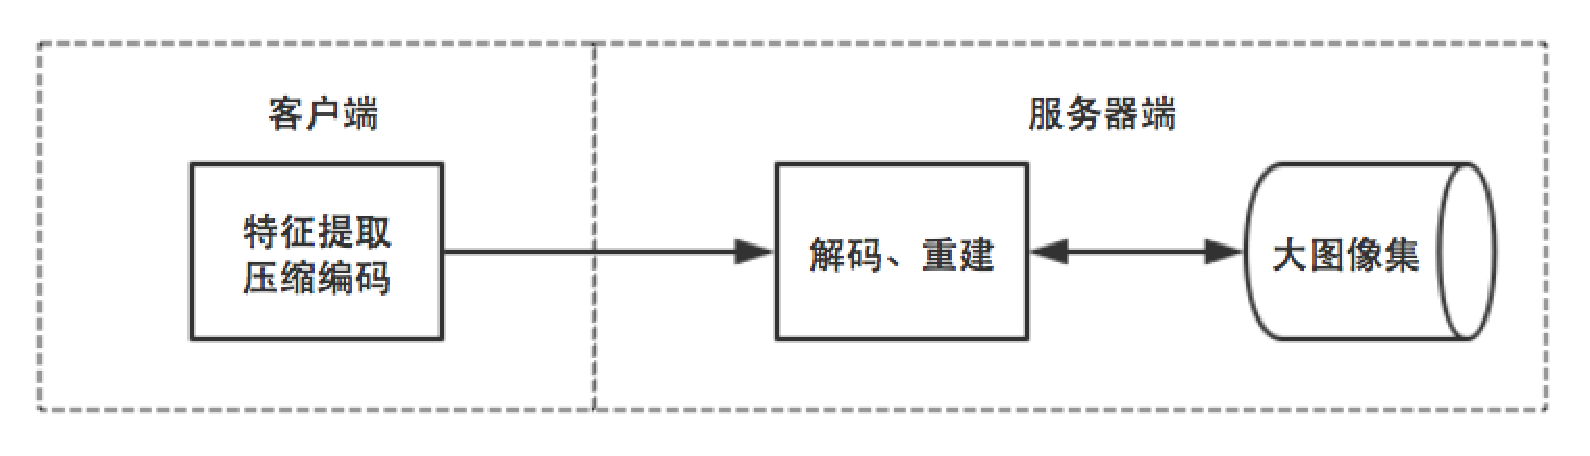
\includegraphics[width=14cm]{imgs/ch1/overview}
\caption{基于与的图像压缩模式}
\label{fig:overview}
\end{figure}
这种架构所运用的核心技术手段便是基于局部特征的图像重建算法,通过对原始图像的特征提取与重建,利用计算资源减少带宽损耗,从一个全新的维度进行数据压缩,为多媒体应用开启了一扇大门。

\section{国内外研究现状}

本文所探讨的基于局部特征的图像重建算法的脱胎于图像拼接技术和相似图像搜索技术,这两个技术相对而言较为成熟:图像拼接领域,SIFT特征的强可区分性和不变性使之广泛应用在全景图拼接领域\cite{Brown:2006ir};相似图像搜索在近年来发展较快,在搜索效率和搜索准确度两个层面进行探索,利用局部特征取代全局特征\cite{Xu:2013wc,POLICY:2013te,Wu:2009bl}以及利用局部特征的空间编码\cite{Zhou:2010tv}进行更为精确的相似图像搜索,使用min-hash等技术对特征进行压缩\cite{Chum:2008jo}提高搜索的速度。

在其上发展而来的基于局部特征的图像重建算法是近几年刚刚提出的一项新颖的技术手段,Philippe Weinzaepfel等人于2011年首先提出了基于局部特征进行图像的重建\cite{Weinzaepfel:2011jh},重建方法首先是根据局部特征使用传统技术在大数据集上找到与原始图像视觉相似的图像块,通过特征匹配与配准将候选图像块转换到标准图像域,通过无缝拼接技术将其拼合在一起,最后使用平滑差值计算空白区域的像素值,以椭圆形图像块为基本单元,重建的结果如图\ref{fig:Weinzaepfel_res}所示。

\begin{figure}
\centering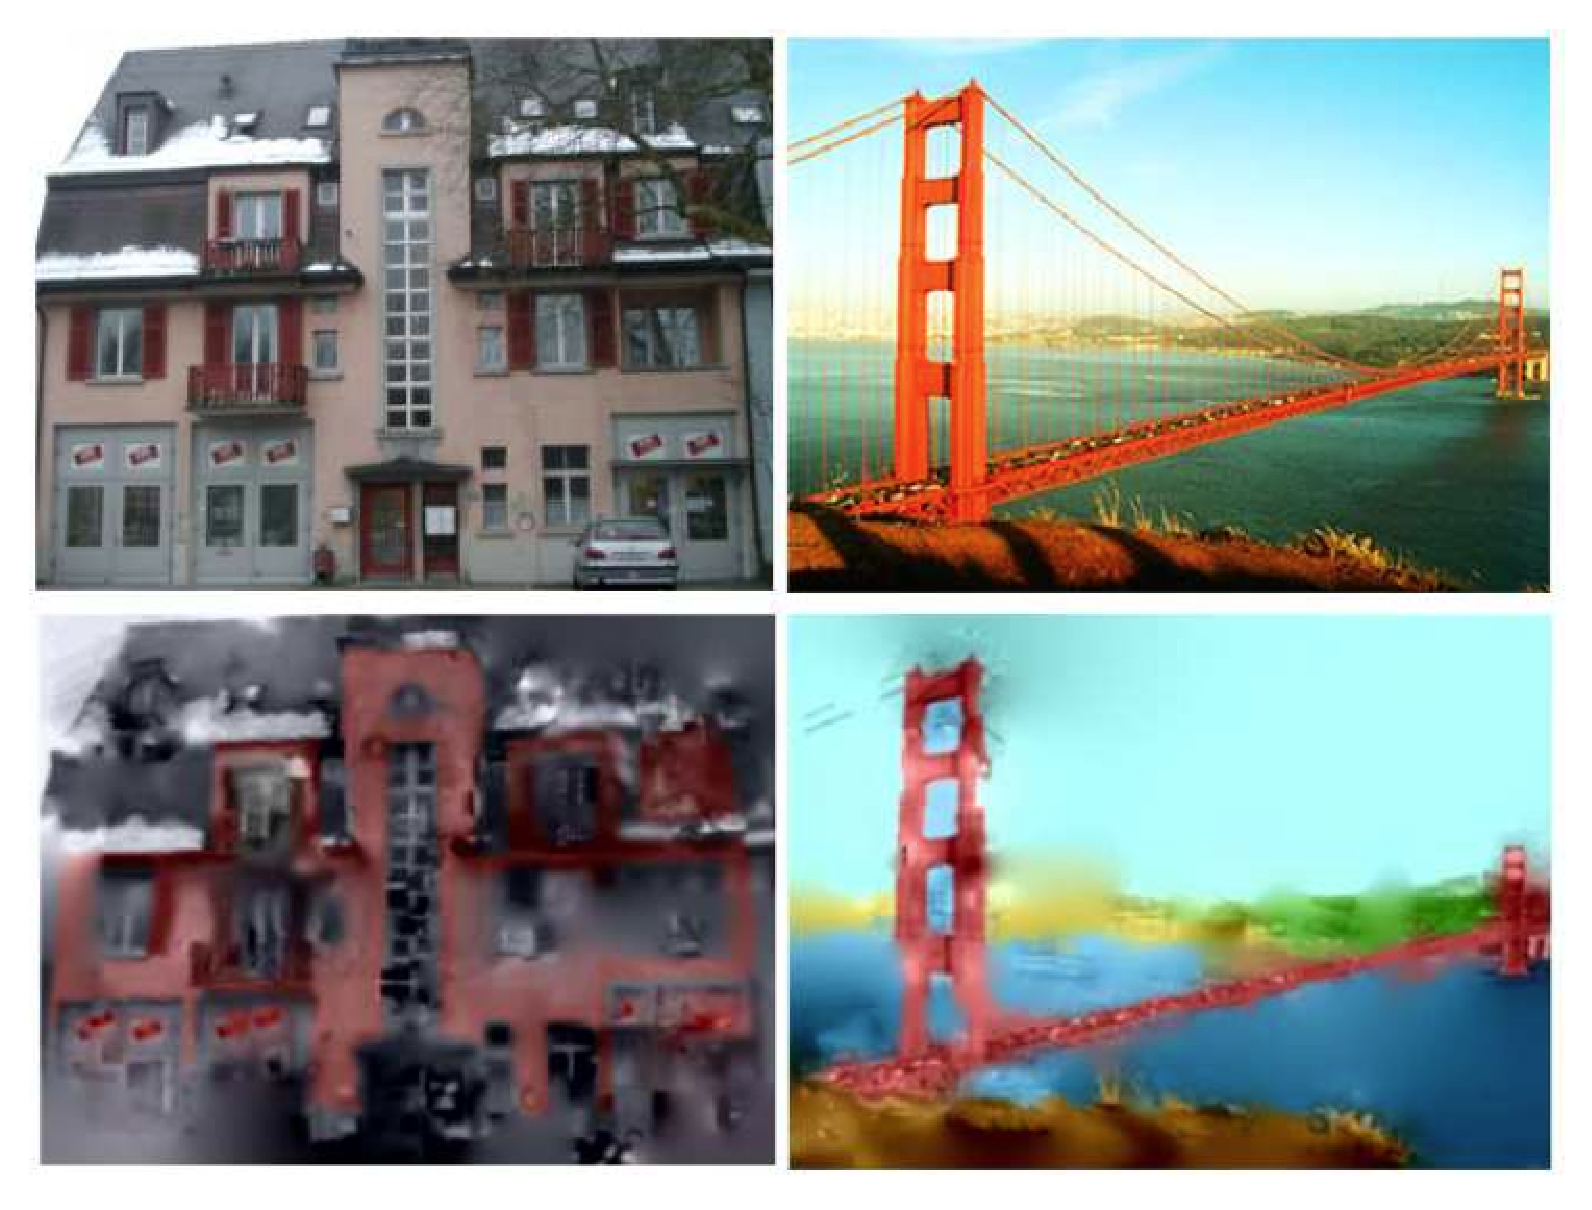
\includegraphics[width=15cm]{imgs/ch1/Daneshi_res}
\caption{Daneshi基于局部特征的图像重建结果}
\label{fig:Daneshi_res}
\end{figure}

在这一自动化的图像重建系统中,虽然重建结果没有达到视觉满意程度,但是显示了基于特征进行重建的可能性,作者由此提出了图像的局部特征信息可能泄露用户隐私这一话题。

随后,Maryam Daneshi和Jiaqi Guo\cite{Daneshi:2011wi}则在确实特征尺度信息的前提下,挖掘图像重建的最大可能。他们采用方形图像块作为重建的基本单元,利用贪婪算法逐步的学习每一个图像块的尺度,完成图像的亮度信息重建,最后采用用户指定颜色遮罩并用最优化算法来进行上色,重建结果如图\ref{fig:Daneshi_res}所示,重建结果保留了大部分的图像信息。

\begin{figure}
\centering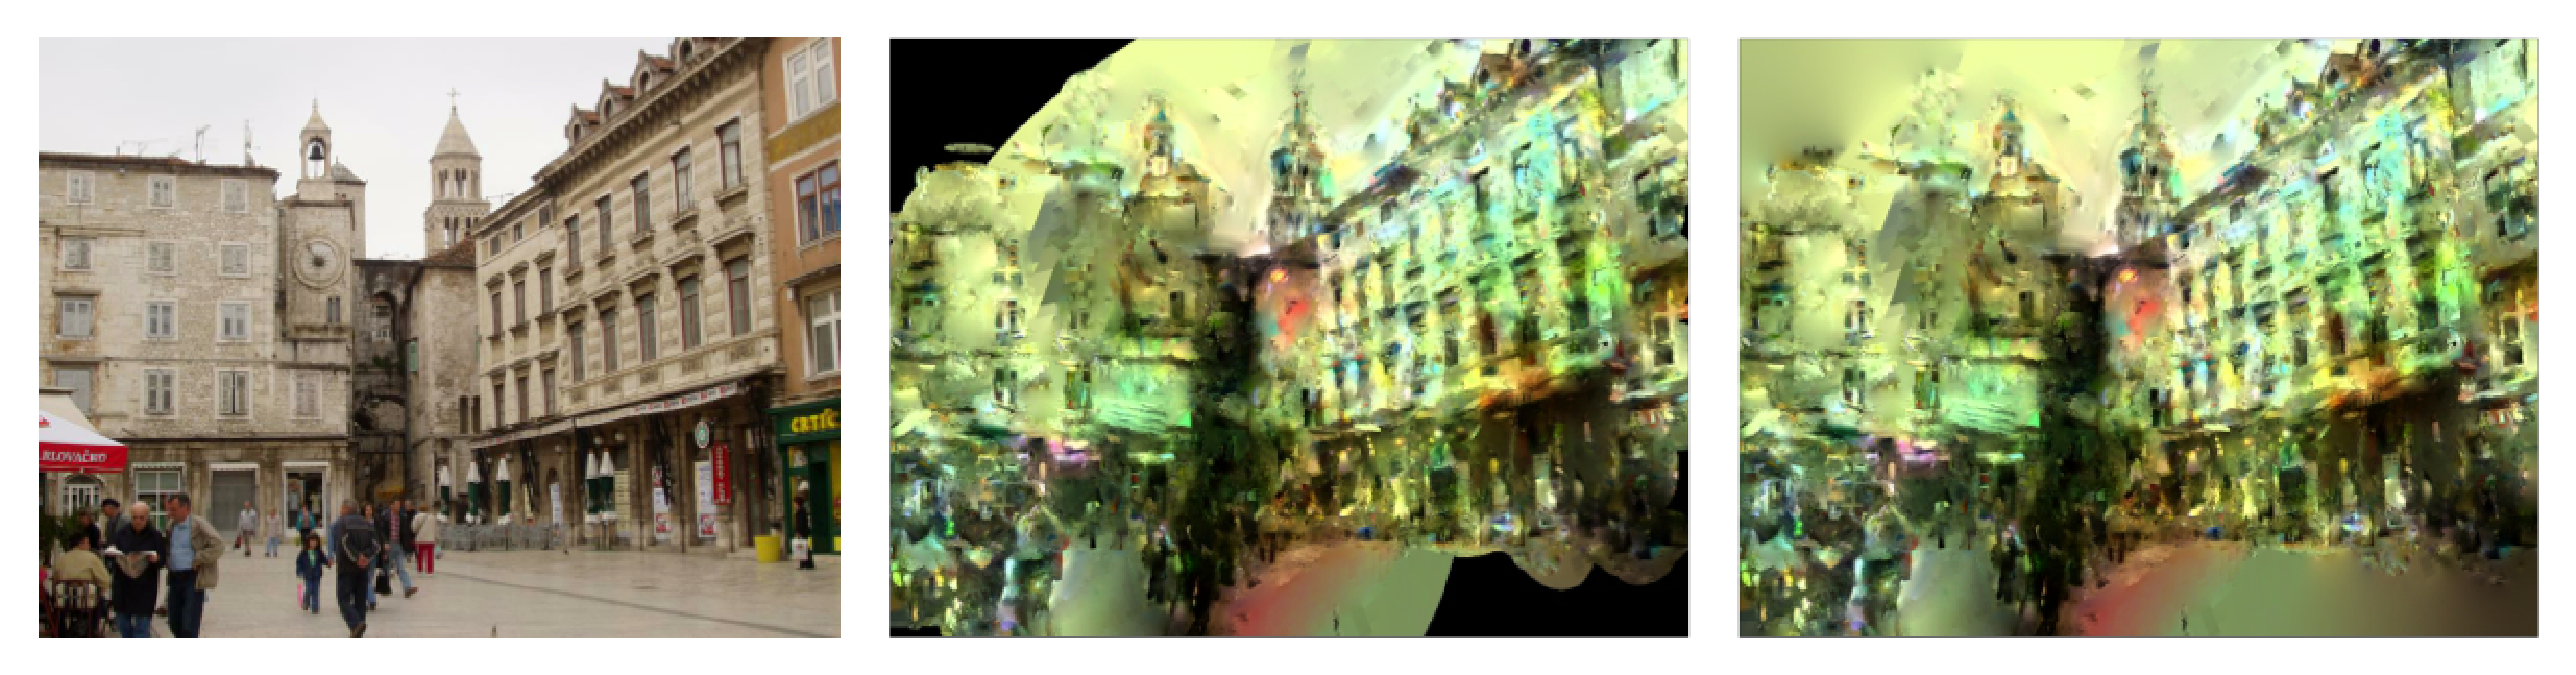
\includegraphics[width=15cm]{imgs/ch1/Weinzaepfel_res}
\caption{Weinzaepfel基于局部特征的图像重建结果,从左向右依次是原始图像、重建图像、补全后的图像}
\label{fig:Weinzaepfel_res}
\end{figure}

Lican Dai等人提出将其应用在手机地标图像的实时分享\cite{Dai:2012vn},采用基于搜索的重建技术搭建了IMShare系统,提出使用缩略图来指导服务器端的特征提取和图像融合,实验结果显示缩略图的使用大大提升了图像的重建结果,该系统不仅能够重建人眼视觉满意的图像,而且采用并行的处理手段,能在秒这一数量级上完成重建流程。Huanjing Yue使用相似的技术手段进行超分辨率的图像生成,使用低分辨率(LR)的图像在大数据集上进行搜索,得到高分辨率(HR)的候选图像,再通过特征提配与图像重建的技术手段生成超分辨率图像(SR)。

综上所述,基于局部特征的图像重建算法是一项较新的领域,将其用在图像在客户端和服务器端压缩传输更是一个全新的领域,有着大量的技术难点需要攻克,本文主要是在这一应用场景下,对其中的各种技术手段做进一步的探索。

\section{论文的主要研究内容与章节安排}
\subsection{主要研究内容}

本课题以文献\cite{Yue:2013gl}提出的核心任务与技术框架为基础,重点研究在基于云的图像压缩应用场景下的基于局部特征的图像重建算法,进一步探索利用更丰富的图像特征信息在大语料集中进行高质量的图像重建,使重建图像质量达到人眼主观效果较好的程度。重建任务的核心是通过局部特征找到与原始图像相似的图像单元以及可靠的图像间对应点集合,进而自动地建立图像之间点与点或区域与区域之间的可靠对应关系,根据对应关系采用一定的算法拼接图像单元。基于局部特征对图像进行重建的技术能够让我们在发送端只传输少量的特征数据,而接收端服务器利用大数据集进行高分辨率图像的还原。文献\cite{Yue:2013gl}创新性的提出了基于云的图像编码方式,核心思想是以客户端进行特征提取,在服务器端利用局部特征在大规模图像集上找到相匹配的图像块,利用计算机视觉相关算法将图像块拼合成一幅完整图像,达到图像重建的目的,其服务体系如图\ref{fig:service}所示。

\begin{figure}
\centering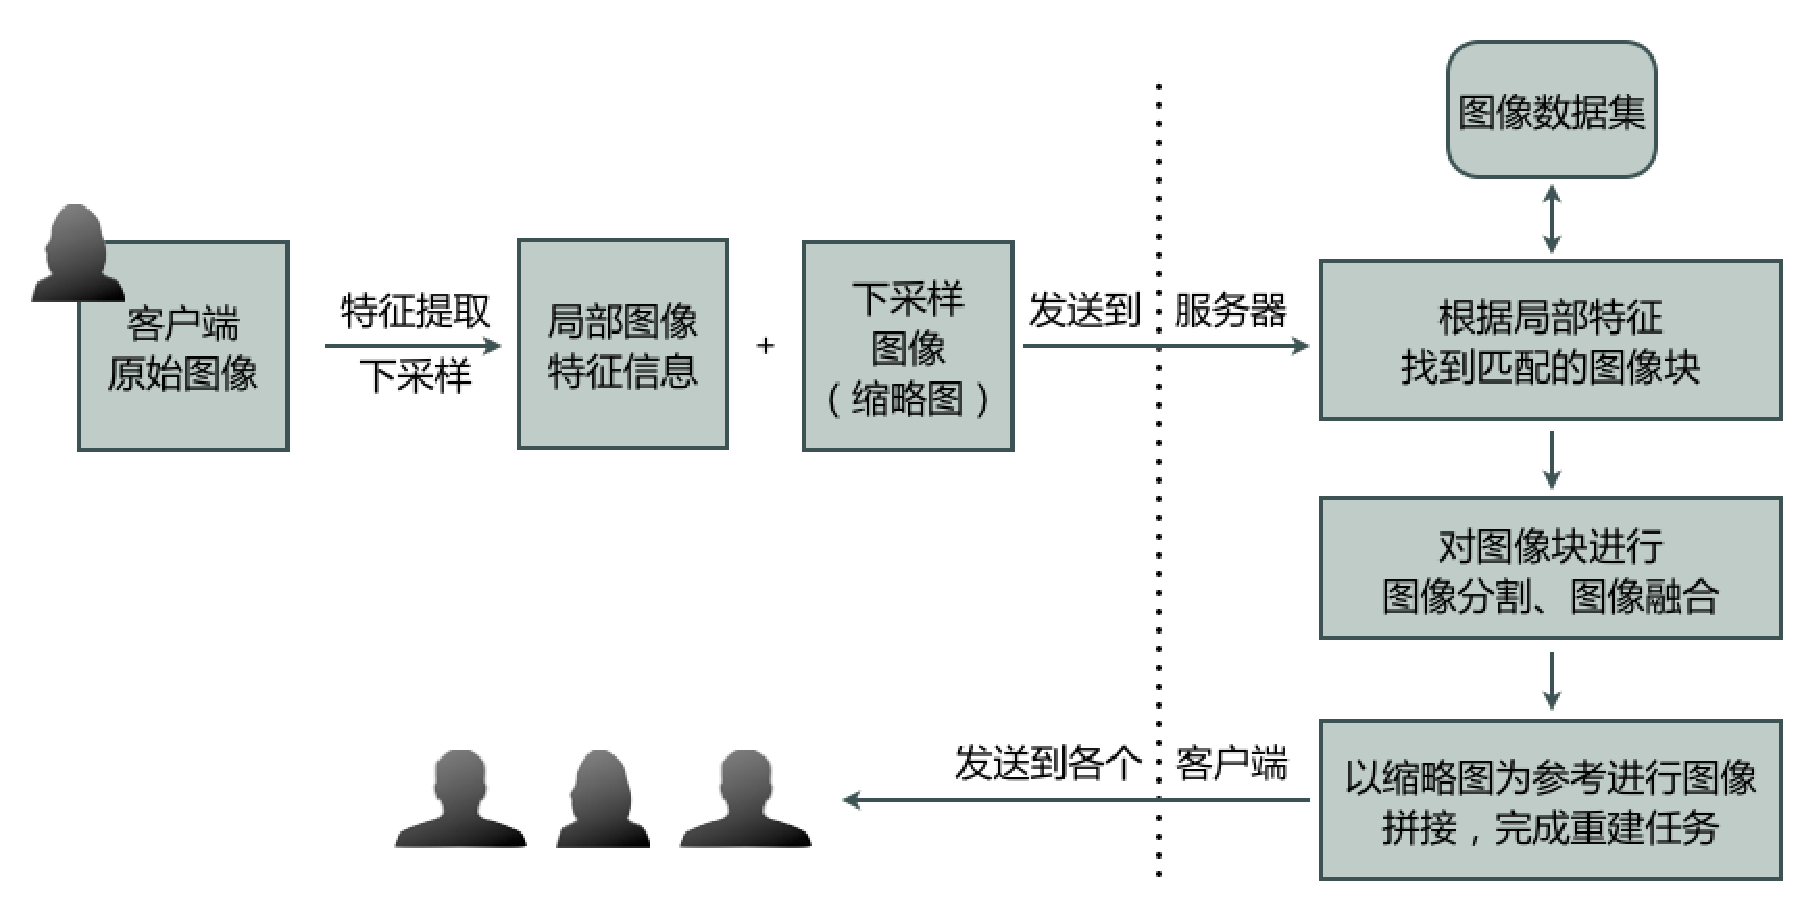
\includegraphics[width=15cm]{imgs/ch1/service}
\caption{基于云压缩的图像服务}
\label{fig:service}
\end{figure}

它主要解决的是在当前手机网络带宽有限的情况下图像的实时分享问题,我国大部分区域还是在2G和3G网络覆盖下,传输一张高分辨率的JPEG图像需要几分钟的时间。并且处理的过程需要占用大量的手机资源,传输的延时和图像分辨率的压缩带来不佳的用户体验。为了解决上述难题,作者提出了基于云压缩的方式进行图像传输:在手机端,下采样获取手机图像的缩略图,使用特征检测与特征描述获取SIFT特征。利用缩略图压缩SIFT算子,经过压缩后,每幅图像能够保持在10KB左右的大小,大大加快了传输速度;在云端有一个大图像数据集,可以通过特征描述借用数据集进行图像的重建;最终,重建的结果以不同分辨率的形式分发到其他用户终端上。

本文在上述的大框架下综合使用多种信息检索与图像处理技术,使用了上述系统中相同的数据编解码方式,而对其中的相似图像检索、图像块筛选等核心算法进行了改进与完善,使之更加能够适用于大规模图像集上的图像重建任务,重建结果得到了进一步的优化。

因此,课题将深入研究基于局部特征进行图像重建任务中的各个环节。从技术范畴来说,本课题可以归纳为两个方面:

\begin{enumerate}
\item 一方面是在计算机视觉领域综合运用图像关键点的提取、局部特征描述、特征匹配、图像配准、图像分割、图像融合等图像处理算法,形成一套完整的基于局部特征进行图像重建的算法流程;
\item 另一方面是针对大数据集的处理,由于图像的匹配与重建等相关任务是建立在大数据集基础之上的,所以本课题试图探索如何在大规模图像集上优化现有的图像重建方案,拟采用改进的聚类算法生成视觉词,利用k-d树等数据结构组织视觉词并进行快速的词条匹配,探索重建任务的并行解决方案。
\end{enumerate}


\subsection{章节安排}
本文分为五个章节,具体内容为:

第一章 绪论。综合论述了立题的意义、背景和课题价值,基于局部特征的数字图像重建算法国内外的研究现状及进展,并进行了归纳,提出了本文研究的应用场景及相关技术,最后总结了本文的章节结构。

第二章 系统概述。主要介绍图像重建算法在基于云的压缩这一场景下的使用。着重介绍本文的系统整体框架,各个模块的输入输出与所使用的技术和算法。

第三章 基于局部特征的图像重建算法。三、四章从两大主要技术环节出发,深入探讨系统所使用的具体算法。第三张从传统的局部特征着手,探讨了图像的匹配、配准、融合等技术手段,并针对大语料集的重建任务对上述算法做了优化与完善。

第四章 大规模近似重复图像搜索算法。探讨系统中所使用的相似图像搜索技术,探讨了从传统的全局特征搜索到局部特征搜索的的发展状况,分析了近期局部特征的使用在相似图像搜索领域的新的发展,从算法的搜索效率与搜索结果多样化两方面对算法进行优化。

第五章 总结与展望。本章总结了目前的工作成果,并对今后基于局部特征的相似图像搜索的研究方向进行了探讨。

%% 本章参考文献
\ifx\usechapbib\empty
\nocite{BSTcontrol}
\bibliographystyle{buptgraduatethesis}
\bibliography{bare_thesis}
\fi
